\documentclass{IOS-Book-Article}

\usepackage{mathptmx}
\usepackage{soul}\setuldepth{article}

\usepackage[gen]{eurosym}
\usepackage{graphicx}
\usepackage{amsmath}

%\usepackage{times}
%\normalfont
%\usepackage[T1]{fontenc}
%\usepackage[mtplusscr,mtbold]{mathtime}
%
\def\hb{\hbox to 11.5 cm{}}

\begin{document}
	
	\pagestyle{headings}
	\def\thepage{}
	\begin{frontmatter}              % The preamble begins here.
		
		
		%\pretitle{Pretitle}
		\title{Bayesian optimization with additive kernels for the calibration of simulation models to perform cost-effectiveness analysis}
		
		\markboth{}{April 2023\hb}
		%\subtitle{Subtitle}
		
		\author[A,B,C]{\fnms{David} \snm{Gómez}\orcid{0000-0003-1787-6482}%
			\thanks{Corresponding Author: David Gómez, dgomez\_ext@iconcologia.net}},
		\author[A,B,C]{\fnms{Mireia} \snm{Díaz}\orcid{0000-0001-9360-4548}}
		\author[D]{\fnms{Josep Lluís} \snm{Arcos}\orcid{0000-0001-7751-1210}}
		and
		\author[D]{\fnms{Jesus} \snm{Cerquides}\orcid{0000-0002-3752-644X}}
		
		%\runningauthor{B.P. Manager et al.}
		\address[A]{Universitat Autònoma de Barcelona (UAB)}
		\address[B]{Institut Català d'Oncologia (ICO)}
		\address[C]{Institut d'Investigació Biomèdica de Bellvitge (IDIBELL)}
		\address[D]{Institut d'Investigació en Intel·ligència Artificial - Consell Superior d'Investigacions Científiques (IIIA-CSIC)}
		
		\begin{abstract}
			Cost-effectiveness (CE) modeling is an essential tool in medicine for evaluating the balance between health benefits and economic sustainability of new health strategies compared to current practices. One critical aspect of these models is the accurate representation of the disease's natural history, which requires a set of parameters such as probabilities and disease burden rates. While these parameters can be obtained from scientific literature, they often need calibration to fit the model's expected outcomes. However, the calibration process can be computationally expensive and traditional optimization methods can be time-consuming due to relatively simple heuristics that may not even guarantee feasible solutions.
			In this work, we investigate the use of Bayesian optimization to enhance the calibration process by leveraging domain-specific knowledge and exploiting inherent structural properties in the solution space. Specifically, we examine the effect of additive kernel decomposition and constraint handling for efficient search. Potential future enhancements also include prior specification for parameters and GPU-friendly computation, among others.
			Our preliminary results show that this improved Bayesian optimization procedure asymptotically improves the calibration process, leading to faster convergence and better solutions for larger CE models.
		\end{abstract}
		
		\begin{keyword}
			bayesian optimization\sep gaussian processes\sep additive kernels\sep constrained optimization\sep simulation models\sep cost-effectiveness models\sep  cancer research
		\end{keyword}
	\end{frontmatter}
	\markboth{April 2023\hb}{April 2023\hb}
	%\thispagestyle{empty}
	%\pagestyle{empty}
	
	\section{Introduction}
	
	\section{Background}
	\subsection{Cost-effectiveness analysis}
	Healthcare decision-making is a challenging task, especially in settings with limited resources. Cost-effectiveness analysis (CEA) is a crucial tool in this context, enabling us to assess the value of healthcare interventions and determine which ones offer the best value for money. By comparing the costs and benefits of alternative interventions, policymakers and healthcare providers can prioritize interventions and allocate resources to achieve the maximum health benefits for the population. Ultimately, the goal of healthcare is to improve health outcomes, and CEA plays a vital role in achieving this objective.
	
	CEA relies on simulation models that mimic disease processes to evaluate the effects of different medical strategies on health outcomes as a group of individuals traverse through different health states (figure \ref{fig:lung_model}). These models can generate various outcomes, but they always produce two critical measures: the average cost and the average life expectancy, usually measured in Quality-Adjusted Life Years (QALYs). By comparing the incremental cost-effectiveness ratio (ICER) of two strategies (equation \ref{eq:icer}), we can determine the additional expenditure required to increase life expectancy by one year if the second strategy is adopted. This ICER can then be compared to a willingness-to-pay threshold determined by the geographical region, with strategies with ICERs falling below the threshold considered cost-effective.
	
	\begin{equation}
		\label{eq:icer}
		\textnormal{ICER}=\frac{\Delta \textrm{Cost}}{\Delta \textrm{Effectiveness}} = \frac{C_2-C_1}{E_2-E_1} \quad [\euro{}/\textrm{QALY}]
	\end{equation}
	
	In order to execute the simulations, input parameters are required to describe the disease process, such as probabilities, hazard ratios, or disease burden rates. Due to the inherent uncertainty of these values, it is often necessary to calibrate the model before proceeding with the analysis. Calibration consists in adjusting the input parameters until the resulting output approximates a target value identified in the scientific literature, such as disease incidence, prevalence, or mortality. This optimization process can be especially taxing for complex models, and may necessitate the use of advanced techniques to efficiently explore the solution space.
	
	Moreover, calibrations can be highly dimensional problems with many arbitrary constraints between parameters, dictated by the specific medical domain. In this work, we explore the challenges associated with calibrating CE models and propose methods to overcome them. By improving the calibration process, we can obtain more accurate estimates of the cost-effectiveness healthcare interventions, thereby supporting policymakers and healthcare providers in their decision-making.
	
	\subsection{Bayesian optimization}
	Bayesian optimization is a widely used technique for optimizing black-box, expensive-to-evaluate functions\cite{bayesian-opt} in a wide range of applications, including machine learning, computer vision, robotics and drug discovery, among others. It is a sequential model-based approach that uses a probabilistic model to iteratively encapsulate our knowledge about the target function and using it to guide the optimization process. This surrogate model starts with a prior distribution, which reflects our initial assumptions about the function, and is updated as new data is gathered. The acquisition function, which measures the promise of a new observation and directs how the search space should be explored, is maximized to identify the next point to evaluate. This process is repeated until a satisfactory solution is found, or a termination criterion is met.
	
	One popular choice for surrogate models are Gaussian Processes\cite{gaussian-processes}. These non-parametric regression models represent each observation as a random variable drawn from a Gaussian distribution $f(x) \sim \mathcal{N}(\mu(x), k(x,x))$. The mean function $\mu(x)$ and the covariance function $k(x,x')$ define the expected value of the Gaussian Process and the degree of dissimilarity between different inputs, respectively. For an assumed noise level in the data $\sigma^2$, an initial prior $\mu_0(X)$ (often $\mu_0(X)=0$), a given observation set $X=\{\vec{x_1}, ..., \vec{x_D}\}$ with labels $\vec{y}$ and a Gram matrix $K$ built from $X$ and a set of unknown observations $X_*$, a Gaussian Process $f_*$ has an analytic form for the predictive posterior distribution (equation \ref{eq:predictive_posterior}) and the marginal loglikelihood function (equation \ref{eq:loglikelihood}).
	
	\begin{equation} \label{eq:predictive_posterior}
		\begin{aligned}
			f_*|X,\vec{y},X_* & \sim \mathcal{N}(\mu(X_*), \Sigma(X_*)) \\
			\mu(X_*) & = \mu_0(X_*) + K(X_*,X)(K(X,X) + \sigma^2 I)^{-1}(\vec{y} - \mu_0(X_*)) \\
			\Sigma(X_*) & = K(X_*,X_*) + \sigma^2 I - K(X_*,X)(K(X,X) + \sigma^2 I)^{-1} K(X,X_*)
		\end{aligned}
	\end{equation}
	
	\begin{equation} \label{eq:loglikelihood}
		\begin{aligned}
			\log{p(\vec{y}|X)} &= -\frac{1}{2}\vec{y}^T (K(X,X) + \sigma^2 I)^{-1}\vec{y} - \frac{1}{2}\log{|K(X,X) + \sigma^2 I|} - \frac{n}{2}\log{2\pi}
		\end{aligned}
	\end{equation}
	
	\begin{equation}
		\begin{aligned}
			K(X,X') &= K\left(\begin{bmatrix} \vec{x_1} \\ \vdots \\ \vec{x_m} \end{bmatrix}, \begin{bmatrix} \vec{x'_1} \\ \vdots \\ \vec{x'_n} \end{bmatrix}\right) = \begin{bmatrix} 
				k(x_1,x'_1) & \dots  & k(x_1,x'_n)\\
				\vdots & \ddots & \vdots\\
				k(x_m,x'_1) & \dots  & k(x_m,x'_n)
			\end{bmatrix}
		\end{aligned}
	\end{equation}
	
	The covariance function or kernel is the mechanism to give a Gaussian Process its expressive power, and its choice will heavily depend on the kind of function we aim to model\cite{kernel-composition}. The squared exponential (SE) kernel $k(x,x') = \sigma^2 e^{-\frac{||x-x'||^2}{2l^2}}$ is a popular choice, despite significant drawbacks such as its locality and sensitivity to the curse of dimensionality\cite{curse-dimensionality}. As a result, the SE kernel can be an inefficient option in many high-dimensional Bayesian Optimization problems.
	
	Many techniques are under active research to address high-dimensional problems with Gaussian Processes\cite{gp-high-dim}\cite{gp-high-dim2}. One of these techniques is additive kernel decomposition\cite{gp-additive}. The full additive kernel is shown in equation \ref{eq:additive1} as the weighted sum of the additive kernels of all order interactions (equation \ref{eq:additive2}), when a SE kernel is used as the base kernel (equation \ref{eq:additive3}).
	
	\begin{equation} \label{eq:additive1}
		\begin{aligned}
			k_{add}(x,x') &= \sum_{i=1}^D{\sigma_i^2 k_{add_i}(x_i,x_i')}
		\end{aligned}
	\end{equation}
	
	\begin{equation} \label{eq:additive2}
		\begin{aligned}
			k_{add_j}(x,x') &= \sum_{1\leq i_1 < i_2 < \ldots < i_j\leq D} \left[\prod_{d=1}^{j} k_{i_d}(x_{i_d},x_{i_d}') \right]
		\end{aligned}
	\end{equation}
	
	\begin{equation} \label{eq:additive3}
		\begin{aligned}
			k_i(x,x') &= e^{\frac{(x_i-x_i')^2}{2l_i^2}}
		\end{aligned}
	\end{equation}
	
	Additive kernels suffer from the non-identifiability problem for summed functions. To ensure a unique decomposition, Lu et al\cite{gp-additive-orthogonal} proposed an extension of additive kernels by including an extra constant kernel with an additional variance hyperparameter $\sigma_0^2$ and an orthogonality constraint to generate Orthogonal Additive Kernels (OAK)\cite{gp-additive-orthogonal}. Assuming a normal input distribution $x_i \sim \mathcal{N}(\mu_i, \delta_i^2)$, the following constrained base kernel is derived:
	
	\begin{equation} \label{eq:additive-orthogonal}
		\begin{aligned}
			k_{add_{OAK}}(x,x') &= \sum_{i=0}^D{\sigma_i^2  \tilde{k}_{add_i}(x_i,x_i')} \\
			\tilde{k}_{add_0}(x,x') &= 1\\
			\tilde{k}_{add_j}(x,x') &= \sum_{1\leq i_1 < i_2 < \ldots < i_j\leq D} \left[\prod_{d=1}^{j} \tilde{k}_{i_d}(x_{i_d},x_{i_d}') \right]\\		
			\tilde{k}_i(x,x') &= e^{\frac{(x_i-x_i')^2}{2l_i^2}} - \frac{l_i\sqrt{l_i^2 + 2\delta_i^2}}{l_i^2 + \delta_i^2} e^{-\frac{(x_i-\mu_i)^2 + (x_i'-\mu_i)^2}{2(l_i^2 + \delta_i^2)}}
		\end{aligned}
	\end{equation}
	
	One important advantage of these additive kernels is that we can interpret the $\sigma_i^2$ as the contribution of each individual order to the total kernel. Since many problems often rely on a few low-order interactions, we can truncate the rest of higher orders and limit the computational cost while retaining most of the information present in the full decomposition. To achieve this, OAK kernels can be useful in accurately identifying each contribution and providing an accurate representation on the actual composition on the function.
	
	\section{Methodology}
	\subsection{Cost-effectiveness model}
	We used a lung cancer model used in a published cost-effectiveness analysis\cite{lung-model} as a fast benchmark for Bayesian Optimization on CE models. This Markov-based model simulates a cohort's progression through seven different health states from 35 to 79 years of age, in monthly intervals. The transition probabilities used in the model were age-specific, with distinct values for each 5-year age group (i.e. 35-39, 40-44, ..., 75-79). The state diagram for this model is pictured in figure \ref{fig:lung_model}.
	
	\begin{figure}[h!]
		\centering	
		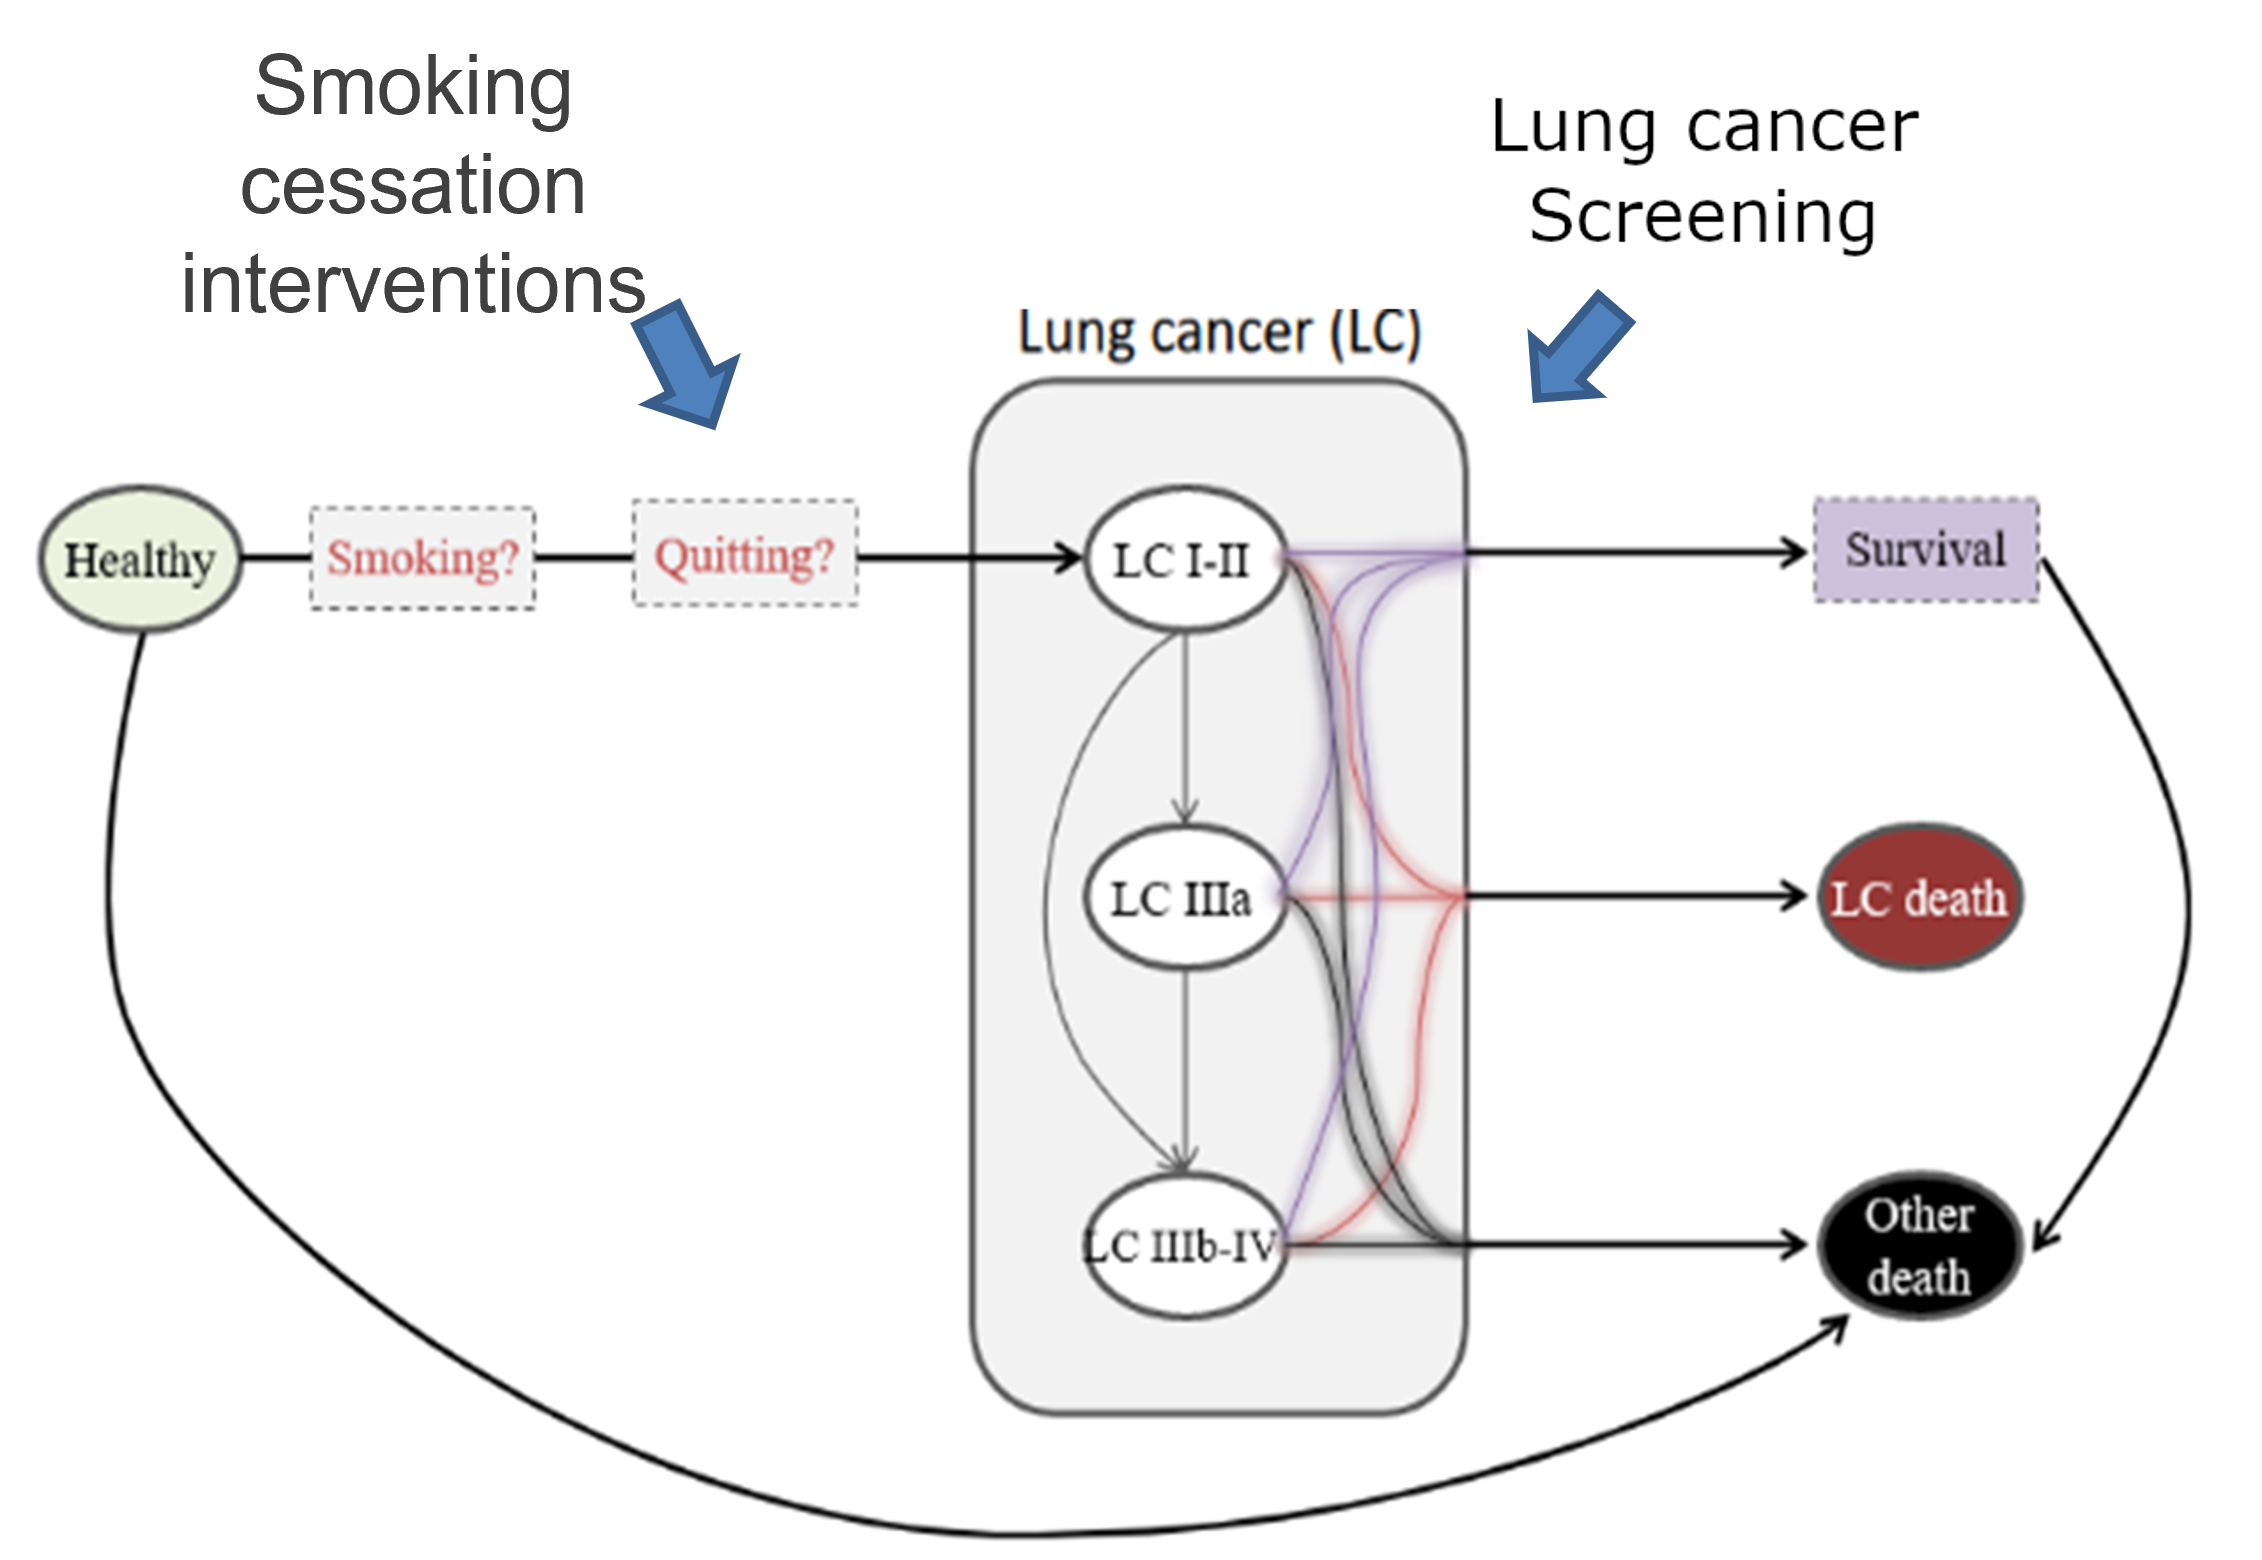
\includegraphics[width=50mm]{figs/lungmodel.png}		
		\caption{Lung cancer markov model state diagram}	
		\label{fig:lung_model}	
	\end{figure}
	
	To simplify the calibration tests, certain details were ignored in the original model, such as gender differentiation, smoking prevalence, and quitting probabilities for smokers. Additionally, the survival state was removed, resulting in only six states being considered and 6x6 transition matrices being used. Certain inherent constraints, such as ensuring that the sum of the probabilities in each row equals one or that certain probabilities are zero, were imposed on the matrices. This allowed the number of parameters to be optimized per matrix to be reduced from 36 to 11. It is worth noting that despite there being 9 age groups, each with its own set of parameters, only the first age group was calibrated in this study. As a result, the problem was simplified to only 11 parameters, rather than the original $11\cdot 9=99$ parameters associated with the full simulation.
	
	The calibration target for the model was defined as the weighted sum of the euclidean distances between the observed and expected outputs of interest, namely lung cancer incidence (45\%), lung cancer mortality (45\%) and mortality from other causes (10\%), computed for each age group.
	
	\subsection{Optimization methods}
	In cost-effectiveness modeling, it is common to have an initial estimate of a good solution based on approximate values found in the scientific literature. For all optimization experiments conducted, a solution space of plus or minus $\pm 50\%$ was considered for each input variable, centered around this initial value.
	
	In the first set of tests we used different optimization methods to illustrate the performance differences between regular bayesian optimization and classical methods. For this purpose we used python implementations of Nelder-Mead\footnote{\url{https://docs.scipy.org/doc/scipy/reference/optimize.minimize-neldermead.html}}, Simulated Annealing (SA)\footnote{\url{https://docs.scipy.org/doc/scipy/reference/generated/scipy.optimize.dual_annealing.html}}, Particle Swarm Optimization (PSO)\footnote{\url{https://pyswarms.readthedocs.io/en/latest/}} and Bayesian Optimization with Gaussian Processes\footnote{\url{https://secondmind-labs.github.io/trieste/1.1.2/index.html}}. The default hyperparameter values were used for these methods, except for PSO where the number of particles was set to 1,000 times the number of matrices used.
	
	After this we developed a new BO implementation with Gaussian Processes from scratch using the R programming language. This implementation was used as a rapid prototyping environment to evaluate different enhancements to the optimization process for our specific cost-effectiveness domain, without being concerned by execution time at this stage. This implementation used the Expected Improvement (EI) acquisition function, with Particle Swarm Optimization to search for its maximum. Finally, both the SE and the OAK kernels were implemented. Runtime optimizations such as GPU use are beyond the scope of this work.
	
	Before starting the BO procedure we learn the lengthscales $l_1, ..., l_D$ and the variances $\sigma_0^1, \sigma_1^2, ..., \sigma_n^2$ of the OAK kernel in a two stage process. In the first stage we maximize the marginal likelihood for each lengthscale separately, and in the second stage we maximize the marginal likelihood for the whole set of variances. This approach allows us to break down a complex task for high-dimensional problems into low-dimensional, manageable problems. This is particularly important when working with larger cost-effectiveness models.
	
	\section{Results}
	The execution times of the minimal version of the lung cancer model presented above were unsurprising. The regular trieste implementation of Bayesian Optimization using Gaussian Processes with SE kernels takes significantly more time than the alternatives, as seen in table \ref{tab:result-methods}.
	
	%Taking a sample of 10,000 executions of the CE model, we observed an average execution time of 2.403 ms per simulation, with a standard deviation of 1.485 ms. This is only a rough estimate, since the overhead introduced by the profiling tools is comparable to the actual measured time. ...
	% TODO: Redo calculations and figure with 5-second simulation
	
	\begin{table}[h!]
		\centering
		%\begin{center}
		\begin{tabular}{llll} 
			\hline
			Method & Error & Time (s) & Evaluations \\ 
			\hline
			Nelder-Mead & 0.663308 & 0.76 & 252 \\ 
			Particle Swarm & 0.66298 & 22.97 & 10100 \\
			Bayesian Optimization & 0.662985 & 114.89 & 21 \\
			\hline
		\end{tabular}
		\caption{Comparison of different optimization methods in the CE model with one age group ($k=1$).}
		\label{tab:result-methods}
		%\end{center}
	\end{table}
	
	In any case, the real focus of our research in this work is the number of evaluations, where we see a sharp drop in error when using BO to achieve a similar level of accuracy compared to other methods, as shown in figure \ref{fig:method_comparison}. Although each iteration requires a significant amount of time due to the bayesian inference step, this overhead obviously will become less relevant as the size of the model increases.
	
	\begin{figure}[h!]
		\centering	
		\includegraphics[width=\textwidth]{figs/methods\_n1.pdf}		
		\caption{Time series of the simplified lung cancer model calibration error (using 1 age group). The error is plotted against the number of evaluations grouped by method. For clarity, the cumulative minimum error is shown.}
		\label{fig:method_comparison}	
	\end{figure}
	
	While exploring the results of Bayesian Optimization with OAK kernels we found that one of the variables had very significant explanatory power by itself, which could produce misleading results in the comparison. To address this issue, we introduced a third univariate SE kernel that considers only this variable. Figure \ref{fig:results_oak} shows the average progression of the error during the optimization process for the three kernels and their confidence interval for a sample of 30 random executions. The univariate SE kernel shows a lower average error and lower deviation than the full SE kernel, due to the reduction in dimensionality of the problem that allows for an easier exploration of the solution space, with barely any information loss. However, the OAK kernel under a normality assumption for the inputs is able to efficiently search the full 11-dimensional space to reach even better average results than the univariate SE kernel, while reducing the deviation as the optimization progresses.
	
	\begin{figure}[h!]
		\centering	
		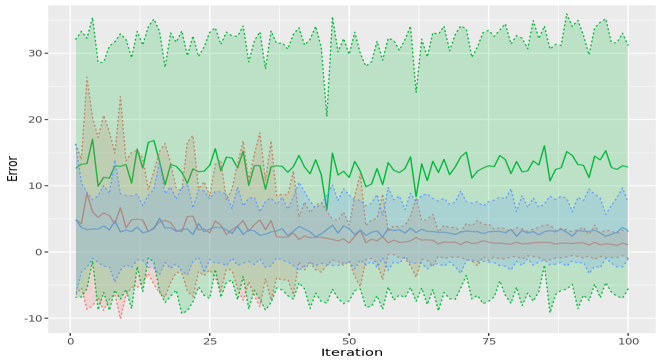
\includegraphics[width=\textwidth]{figs/results.png}		
		\caption{Time series of the error for Bayesian Optimization, using three different kernels: the SE kernel (blue), the univariate SE kernel using only the second variable (green) and the OAK kernel under a normality assumption for the inputs (red).}
		\label{fig:results_oak}	
	\end{figure}
	
	\section{Discussion}
	BO is currently considered a state-of-the-art optimization method in various domains that involve costly functions to evaluate. When the computational cost of the target function is large enough, Bayesian optimization might be the natural choice. But when the function is not as expensive, there are two other critical points in each BO iteration that must be taken into account: the surrogate model regression and the acquisition function optimization.
	
	Regarding the former, SE kernels suffer greatly from the curse of dimensionality. In high-dimensional problems, the number of observations to explore the solution space quickly increases. This renders the regression unfeasible when trying to invert large Gram matrices to calculate the posterior predictive distribution. To address this issue, OAK kernels can reduce the number of necessary observations, mitigate the effects of an expanding Gram matrix and enhance the efficiency of the search.
	
	The optimization of the acquisition function is the initial bottleneck, where the number of observations is still small enough so that the surrogate model regression is not yet a problem. As the search space remains constant, this acquisition optimization doesn't become much more expensive as more data is observed. We used PSO as an easy way to take advantage of parallelism in this area, but other approaches mentioned in the next section are being considered as well\cite{acquisition-functions}.
	
	Lu et al\cite{gp-additive-orthogonal} mention that an interesting direction of work would be to extend OAK kernels to Bayesian Optimization leveraging the inferred low-order representation. In our tests we show that, even with a straightforward application of OAK kernels on this simple example, a slight improvement over the SE kernel is noticeable. This improvement is expected to be more meaningful for complex models, where more structure can be leveraged. It is interesting to note that these results hold even though some assumptions of the model were not met. Specifically, hyperparameter tuning was performed with a dataset sampled from a uniform input distribution, while the constrained kernels were calculated assuming normality in the input. Even if these distributions were consistent we still would have the problem of determining the input distribution for the actual optimization process, which would be neither normal nor uniform.
	
	%gp max likelihood ill-posed -> impose gaussian noise
	
	\section{Future work and conclusions}
	One particular aspect that we didn't incorporate into this article is constraint handling. CE models can be highly constrained problems, and these constraints are another expression of the structure of the solution space. We have been able to manage arbitrary constraints successfully using additional surrogate models and a new Constrained Expected Improvement acquisition function, as introduced by Gardnet et al\cite{gp-constraints}.
	
	We also mentioned in this work the importance of exploiting the parallelization potential of the different areas of the optimization process. For that purpose we use PSO for the optimization of the acquisition function, but other more sophisticated venues for parallelization include batched optimization\cite{gp-batch}\cite{gp-batch2}, parallel acquisition functions\cite{gp-parallel-acq-func} or GPU approaches\cite{gp-gpu} among others.
	
	Our research group recognizes the importance of efficiently calibrating increasingly complex CE models, injecting relevant domain knowledge in the process. The content of this work is only the beginning of several enhancements that are being implemented to have the tools to work with more challenging models in the future.
	
	\begin{thebibliography}{99}
		
		\bibitem{ce-models}
		Kuntz, Karen M. and others, 'Decision Models in Cost-Effectiveness Analysis', in Peter J. Neumann and others (eds), Cost-Effectiveness in Health and Medicine, 2nd edn (New York, 2016; online edn, Oxford Academic, 17 Nov. 2016)
		
		\bibitem{ce-calibration}
		Moriña, D., Díaz, M. (2017). Calibration Approach Impact on Health and Cost-Effectiveness Outcomes in a Decision Analytic Framework. Value in Health, 20(9), A407–A408
		
		\bibitem{bayesian-opt}
		Bergstra, J., Bardenet, R., Bengio, Y., \& Kégl, B. (2011). Algorithms for Hyper-Parameter Optimization. Advances in Neural Information Processing Systems, 24.
		
		\bibitem{gaussian-processes}
		Carl E. Rasmussen and Christopher K. I. Williams. Gaussian Processes for Machine
		Learning. MIT Press, 2006.
		
		\bibitem{kernel-composition}
		Duvenaud, D., Lloyd, J., Grosse, R., Tenenbaum, J. \& Zoubin, G.. (2013). Structure Discovery in Nonparametric Regression through Compositional Kernel Search. Proceedings of the 30th International Conference on Machine Learning, in Proceedings of Machine Learning Research 28(3):1166-1174
		
		\bibitem{curse-dimensionality}
		Bengio Y. (2007). On the challenge of learning complex functions. Progress in brain research, 165, 521–534.
		
		\bibitem{gp-additive}
		Duvenaud, D. K., Nickisch, H., \& Rasmussen, C. (2011). Additive Gaussian Processes. Advances in Neural Information Processing Systems, 24.
		
		\bibitem{acquisition-functions}
		Wilson, J.T., Hutter, F., \& Deisenroth, M.P. (2018). Maximizing acquisition functions for Bayesian optimization. Neural Information Processing Systems.
		
		\bibitem{gp-additive-orthogonal}
		Lu, X., Boukouvalas, A., \& Hensman, J. (2022). Additive Gaussian Processes Revisited. Proceedings of the 39th International Conference on Machine Learning, 14358–14383.
		
		\bibitem{gp-high-dim}
		Durrande, N, Ginsbourger, D \& Roustant, O. Additive Covariance kernels for high-dimensional Gaussian Process modeling. Annales de la Faculté des sciences de Toulouse : Mathématiques, Serie 6, Volume 21 (2012) no. 3, pp. 481-499.
		
		\bibitem{gp-high-dim2}
		Binois, M., \& Wycoff, N. (2022). A Survey on High-dimensional Gaussian Process Modeling with Application to Bayesian Optimization. ACM Transactions on Evolutionary Learning and Optimization, 2(2), 8:1-8:26.
		
		\bibitem{lung-model}
		Diaz, M., Garcia, M., Vidal, C., Santiago, A., Gnutti, G., Gómez, D., Trapero-Bertran, M., Fu, M. (2021). Health and economic impact at a population level of both primary and secondary preventive lung cancer interventions: A model-based cost-effectiveness analysis. Lung Cancer, 159, 153–161
		
		\bibitem{gp-constraints}
		Gardner, J.R., Kusner, M.J., Xu, Z.E., Weinberger, K.Q., \& Cunningham, J.P. (2014). Bayesian Optimization with Inequality Constraints. International Conference on Machine Learning.
		
		\bibitem{gp-batch}
		González, J.I., Dai, Z., Hennig, P., \& Lawrence, N.D. (2015). Batch Bayesian Optimization via Local Penalization. International Conference on Artificial Intelligence and Statistics.
		
		\bibitem{gp-batch2}
		Rontsis, N., Osborne, M. A., \& Goulart, P. J. (2020). Distributionally Ambiguous Optimization for Batch Bayesian Optimization. Journal of Machine Learning Research, 21(149), 1–26.
		
		\bibitem{gp-parallel-acq-func}
		Wang, J., Clark, S. C., Liu, E., \& Frazier, P. I. (2020). Parallel Bayesian Global Optimization of Expensive Functions. Operations Research, 68(6), 1850–1865.
		
		\bibitem{gp-gpu}
		Wang, K. A., Pleiss, G., Gardner, J. R., Tyree, S., Weinberger, K. Q., \& Wilson, A. G. (2019). Exact gaussian processes on a million data points. In Proceedings of the 33rd International Conference on Neural Information Processing Systems (pp. 14648–14659). Curran Associates Inc.
		
	\end{thebibliography}
	
\end{document}
